% !TeX spellcheck = hu_HU
\documentclass[12pt,a4paper]{article}
\usepackage[utf8]{inputenc}
\usepackage{cmap}
\usepackage[T1]{fontenc}
\usepackage[magyar]{babel}
\usepackage{amsmath}
\usepackage{amsfonts}
\usepackage{amssymb}
\usepackage{graphicx}

\usepackage{struktex}
\usepackage{outlines}
\usepackage{hyperref}

\hyphenpenalty=10000

\begin{document}

\begin{center}
	\huge
	Algoritmusok és adatszerkezetek II\\
	\vspace{1mm}
	\LARGE
	Fák témakör jegyzete\\
	\vspace{5mm}
	\large
	Készült Ásványi Tibor előadásai és gyakorlatai alapján\\
	\vspace{5mm}
	Sárközi Gergő, 2021-22-1. félév\\
	Nincsen lektorálva!
\end{center}

\tableofcontents

\pagebreak

\section{AVL fák}

\begin{outline}
	\1 (magasság szerint) kiegyensúlyozott bináris keresőfa
		\2 egy fa kiegyensúlyozott, ha minden csúcsa kiegyensúlyozott
		\2 $*p$ kiegyensúlyozott, ha $|p\to b|\le1$
		\2 $p\to b = h(p\to right) - h(p\to left)$
	\1 AVL fákat láncoltan reprezentálunk
	\1 legyen $n=|t|$ (csúcsok száma) és $h=h(t)$
	\1 $ \lfloor log n \rfloor \le h \le 1,45 \log n \implies h \in \Theta(log n) $
		\2 Felső becslés, alsó határ: $n<2^{h+1} \implies \lfloor log n \rfloor \le h$
		\2 Fibonacci fák: $h$ mélységű, legkisebb méretű KBF-ek (kiegyensúlyozott bináris fák) csúcsainak száma: \\
		$f_0=1$, $f_1=2$, $f_h=1+f_{h-1}+f_{h-2}$ $(h\ge2)$ \\
		Ebből megkapható a $h \le 1,45 \log n$ \\
		$f_h = F_{h+3}-1$ (ahol F a rendes fibonacci sorozat)
	\1 $h(t) \le n-1$
\end{outline}

\begin{table}[h!]
\centering
\begin{tabular}{|l|c|l|}
	\hline
	\multicolumn{1}{|c|}{Függvény} & \multicolumn{1}{|c|}{Komplexitás} & \multicolumn{1}{|c|}{Leírás} \\
	\hline
	search($t:Node^*; k:\mathbb{T}$) : $Node^*$ & $\Theta(\log n)$ & \\
	\hline
	min($t:Node^*$) : $Node^*$ & $\Theta(\log n)$ & ugyan így van max(t) \\
	\hline
	AVLinsert($\&t:Node^*; k:\mathbb{T}; \&d:\mathbb{B}$) & $\Theta(\log n)$ & d igaz, ha nőtt h(t) \\
	\hline
	AVLremMin($\&t,\&minp:Node^*; \&d:\mathbb{B}$) & $\Theta(\log n)$ & d igaz, ha csökkent h(t) \\
	\hline
	AVLdel($\&t:Node^*; k:\mathbb{T}; \&d:\mathbb{B}$) & $\Theta(\log n)$ & d igaz, ha csökkent h(t) \\
	\hline
\end{tabular}
\end{table}

\begin{table}[h!]
	\centering
	\begin{tabular}{|l|}
		\hline
		\multicolumn{1}{|c|}{Node} \\
		\hline
		+ $key : \mathbb{T}$ \\
		+ $b : \{-1,0,1\}$ \\
		+ $left, right : Node^*$ \\
		\hline
		+ $Node() \{left:=right:=\emptyset ; b:=0\}$ \\
		+ $Node(x:\mathbb{T}) \{left:=right:=\emptyset ; b:=0 ; key := x\}$ \\
		\hline
	\end{tabular}
\end{table}

\pagebreak

\subsection{Beszúrás}

\subsubsection{Kiegyensúlyozás beszúrás miatt}

\begin{outline}
	\1 Minden esetben 1 vagy 2 lépés (BESZÚRÁS UTÁN CSAK!)
	\1 Nem változtat az inorder bejáráson (logikus, hiszen keresőfa)
\end{outline}

\begin{figure}[h!]
	\centering
	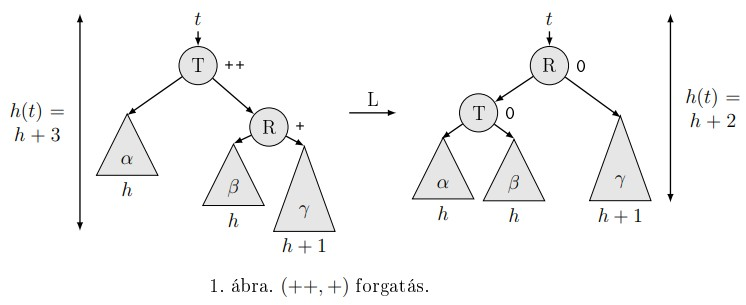
\includegraphics[width=1\linewidth]{forgatas_PPp}
	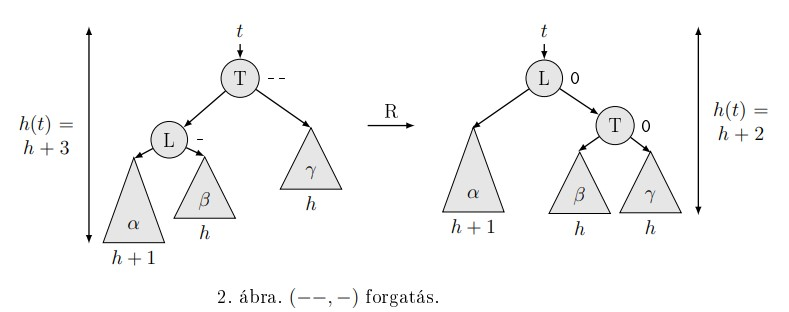
\includegraphics[width=1\linewidth]{forgatas_MMm}
	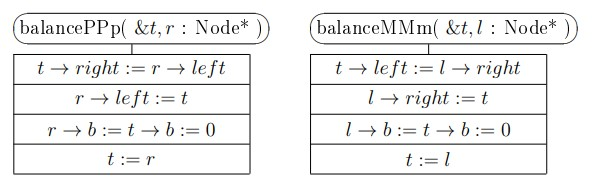
\includegraphics[width=1\linewidth]{balance_PPp_MMm}
\end{figure}

\begin{figure}[p]
	\centering
	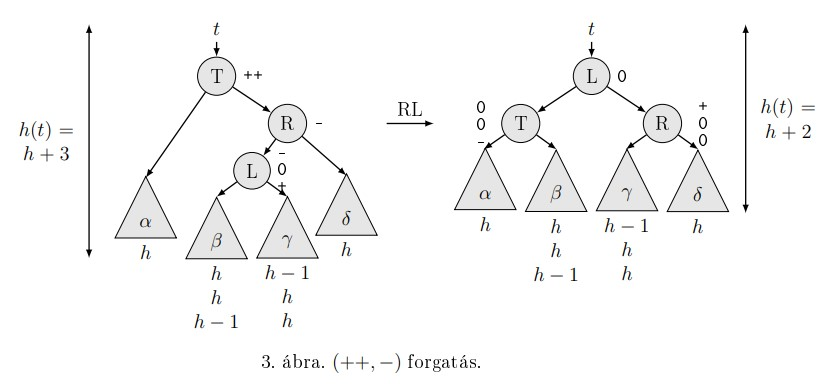
\includegraphics[width=1\linewidth]{forgatas_PPm}
	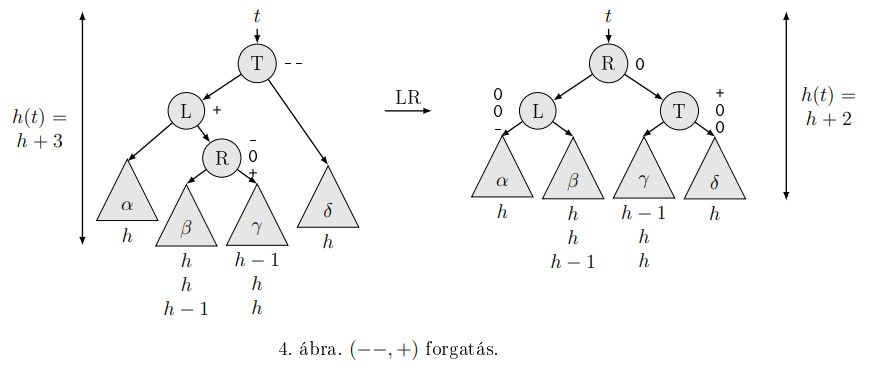
\includegraphics[width=1\linewidth]{forgatas_MMp}
	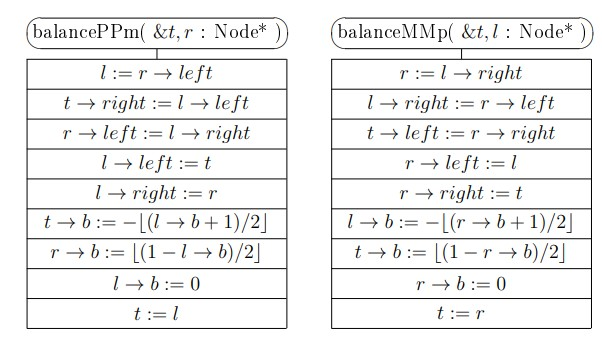
\includegraphics[width=1\linewidth]{balance_PPm_MMp}
\end{figure}

\pagebreak

\subsubsection{Beszúrás algoritmus}

\begin{outline}
	\1 megkeressük a kulcs helyét
		\2 ha a kulcs benne van, kész vagyunk
		\2 ha a kulcs helyén lévő részfa üres: beszúrunk egy levélcsúcsot, így a részfa eggyel magasabb lett
	\1 rálépünk a szülőre és az egyensúlyát módosítjuk (amelyikből ráléptünk, az a gyerek lett eggyel magasabb, szóval balance + vagy - 1)
		\2 ha balance=0, akkor kész vagyunk
		\2 ha |balance|=1, akkor ez a részfa magasabb lett eggyel, ismét rálépünk a szülőre, stb.
		\2 ha |balance|=2, akkor ki kell egyensúlyozni ezt a részfát, miután visszanyeri az eredeti (beszúrás előtti) magasságát, tehát a kiegyensúlyozás után kész vagyunk
\end{outline}

\begin{figure}[h!]
	\centering
	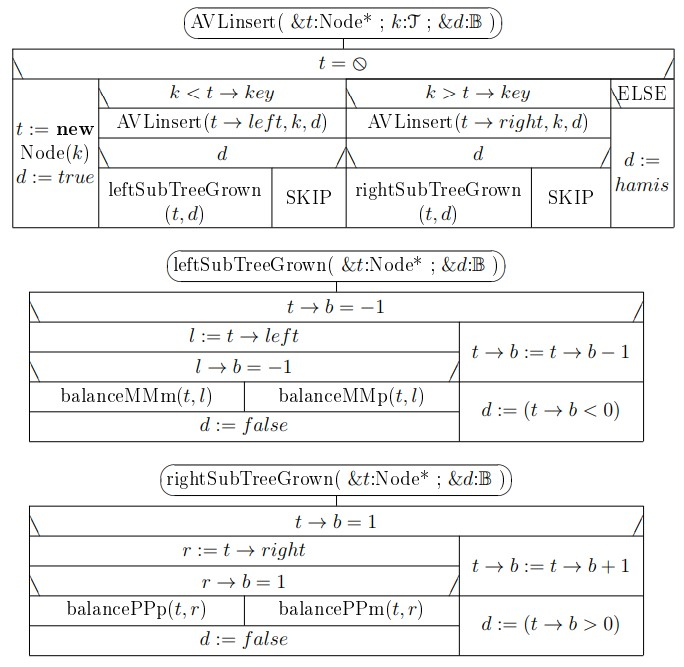
\includegraphics[width=0.8\linewidth]{insert}
\end{figure}

\pagebreak

\subsection{Törlés}

\begin{outline}
	\1 Törlésnél akár több (akár gyökérig tartó) forgatás (kiegyensúlyozás) kell.
	Azért, mert a forgatások csökkentik a részfa magasságát, és a törlés is.
	\1 Törlés fajtái:
		\2 törlendő csúcs egyik részfája üres (levél vagy egy gyerekes csúcs):
		a másik részfát tesszük a csúcs helyére (ami lehet null) és a szülő balance-ját módosítjuk
		\2 kétgyerekes csúcs törlése: jobb részfa minimumjának kiemelése, fa kiegyensúlyozása,
		kicseréljük a törlendő csúcsot a kiemelt csúccsal
\end{outline}

\subsubsection{Kiegyensúlyozás törlés miatt}

\begin{outline}
	\1 Akárhány lépés lehet: forgatások és a törlés is csökkentik a részfa magasságát
	\2 Nem változtat az inorder bejáráson (hiszen keresőfa)
\end{outline}

\begin{figure}[h!]
	\centering
	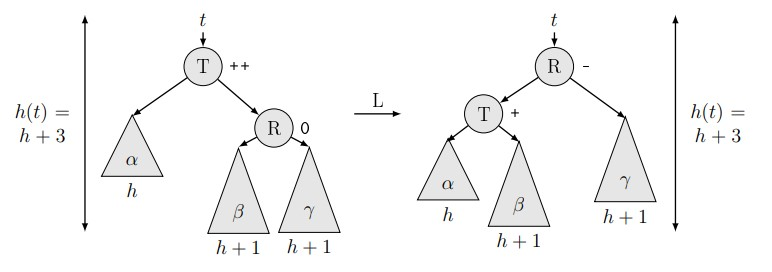
\includegraphics[width=1\linewidth]{forgatas_PP0}
	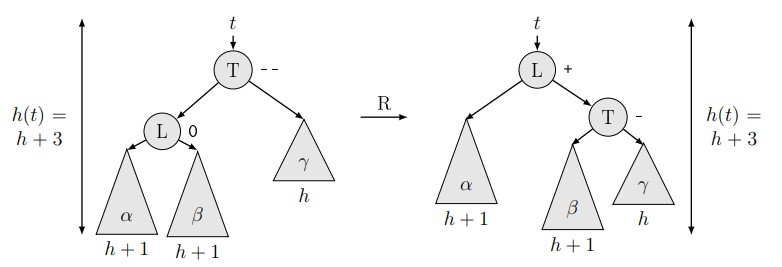
\includegraphics[width=1\linewidth]{forgatas_MM0}
\end{figure}

\begin{figure}[h!]
	\centering
	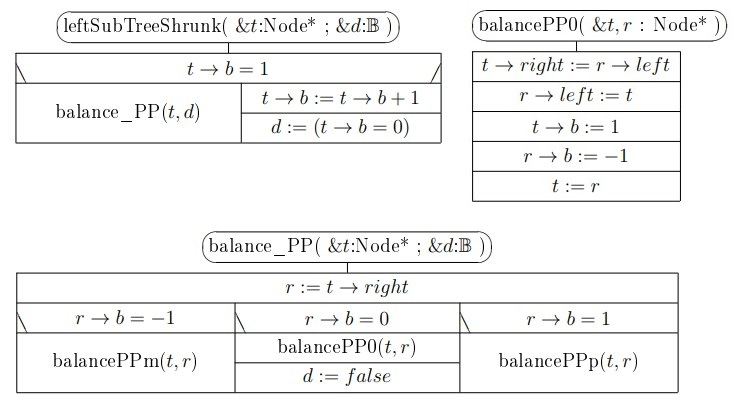
\includegraphics[width=1\linewidth]{balance_PP0}
	TODO balance MM metódus, stb.
\end{figure}

\subsubsection{remMin algoritmus}

\begin{figure}[h!]
	\centering
	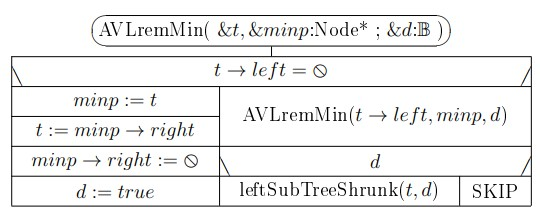
\includegraphics[width=0.7\linewidth]{remMin}
\end{figure}

\pagebreak

\subsubsection{delRoot algoritmus}

\begin{figure}[h!]
	\centering
	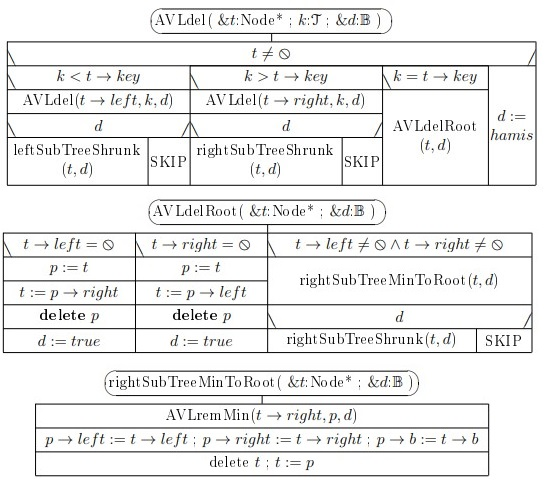
\includegraphics[width=0.9\linewidth]{del}
\end{figure}

\pagebreak

\section{Általános fák}

\begin{outline}
	\1 Csúcsnak tetszőlegesen sok gyereke lehet
	\1 csúcshoz nem tartoznak üres részfák: egy csúcsnak annyi gyereke van, amennyi, nincs üres gyerek
		\2 ezért nem r-áris fákról beszélni
	\1 rendezett fa: ha a gyerekek sorrendje lényeges
	\1 gyökér, levél fogalma ugyan úgy megvan
	\1 $Node$ osztály tagjai: $child1,sibling:Node*$
		\2 létezhetne szülő pointer is
		\2 levél: $p \to child1 = \emptyset$
		\2 utolsó testvér: $p \to sibling = \emptyset$
	\1 szöveges ábrázolás: $(G\; t_1\; t_2\; ...\; t_n)$ (ahol G a gyökér)
\end{outline}


\begin{figure}[h!]
	\centering
	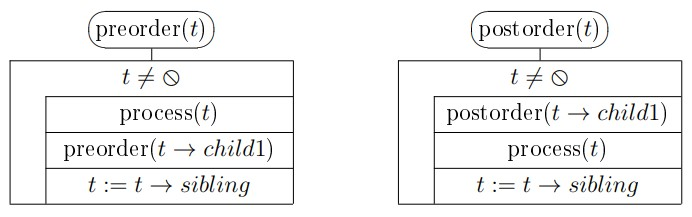
\includegraphics[width=0.9\linewidth]{általános fa bejárás}
\end{figure}

\pagebreak

\section{B+ fák}

\subsection{Felépítés}

\begin{outline}
	\1 $d$ a B+ fa fokszáma, $4 \le d$ (szóval r-áris fa, r=4)
	\1 levelek:
		\2 azonos szinten (mélységben) vannak
		\2 adatokat tárolnak: minden kulcshoz tartozik egy adatra mutató
		\2 szóval a levelekben azonos számú (max $d-1$) kulcs és mutató van
	\1 belső csúcsok:
		\2 max $d$ mutató és pontosan eggyel kevesebb kulcs
		\2 belső kulcsok: hasító kulcsok
		\2 kulcsok viszonya egymáshoz:
			\3 legyen $n$ a részfák száma, $k$ a részfa bármelyik kulcsa
			\3 legyen $K_i$ a szülő $i$. kulcsa ($1 \le i < n$)
			\3 legszélső bal részfa: $k < K_1$
			\3 legszélső jobb részfa: $K_{n-1} \le k$
			\3 közbülső, $i$. részfa: $K_{i-1} \le k < K_i$
	\1 gyerekek száma: (mindig max $d$)
		\2 gyökér: min 2, vagy pontosan 0
		\2 minden nem gyökér belső csúcs: min $\lfloor d/2 \rfloor$
	\1 B+ fa által reprezentált adathalmaz minden értéke megjelenik egy levél kulcsaként, balról jobbra szigorúan monoton növekvő sorrendben
\end{outline}

\subsection{Műveleti igény}

\begin{outline}
	\1 Keresés, beszúrás, törlés: $\Theta(\log n)$
\end{outline}

\pagebreak

\subsection{Beszúrás}

\begin{outline}
	\1 Üres a fa: készítsünk gyökeret, tartalmazza az értéket
	\1 Keressük meg a levelet. Ha a levélben már szerepel a csúcs, fail.
	\1 Ha nincs már a fában a kulcs és nem üres a fa:
		\2 Ha a csúcsban van szabad hely, láncoljuk be oda rendezetten
		\2 Ha a csúcs tele van, vágjuk szét két csúccsá, felezve az elemeket\\
		(elemek közé sorolva az újat is) (ha páratlan: balra menjen több)
			\3 szúrjuk be a jobb oldali csúcs legkisebb értékét a szülőbe
				\4 ha nincs szülő (gyökérben vagyunk), hozzuk létre
				\4 ha nem levél, akkor töröljük a régi helyről
			\3 beszúrás miatt rekurzívan ismételni, amíg szükséges
\end{outline}

\begin{figure}[h!]
	\centering
	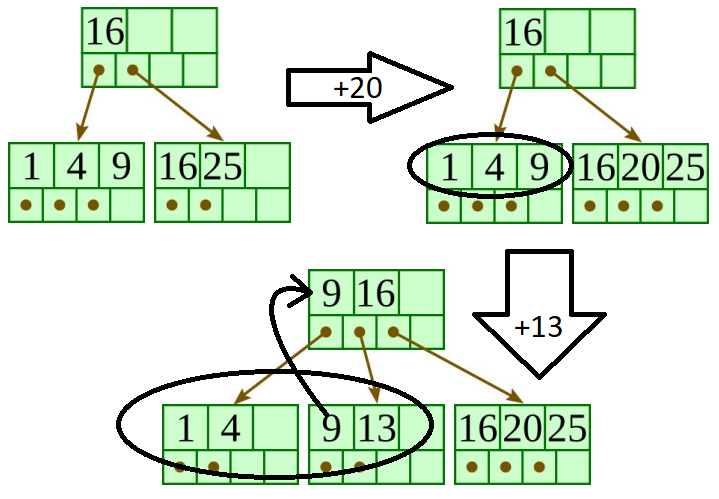
\includegraphics[width=0.5\linewidth]{b+ beszúrás egyszerű}
\end{figure}

\begin{figure}[h!]
	\centering
	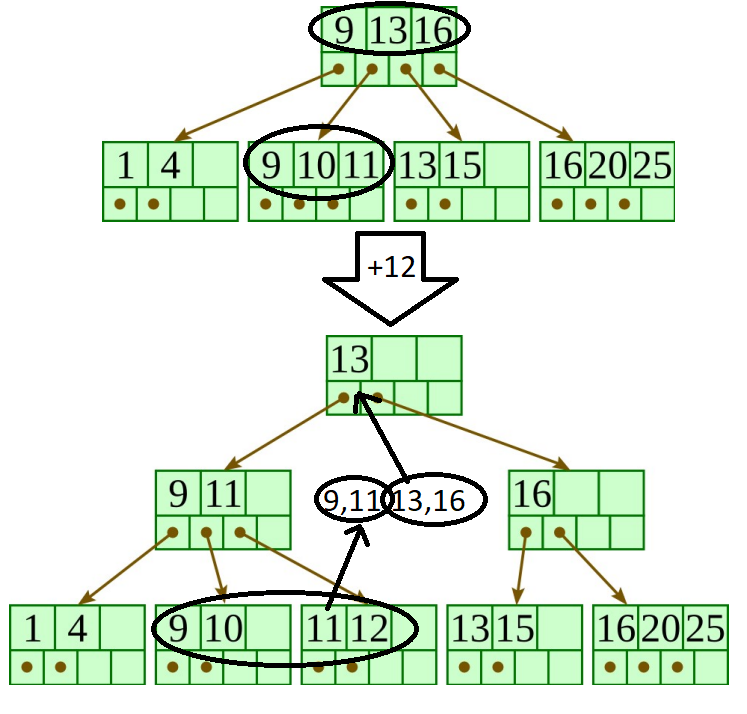
\includegraphics[width=0.5\linewidth]{b+ beszúrás bonyolult}
\end{figure}

\pagebreak

\subsection{Törlés}

Meg kell keresni a törlendő kulcsot tartalmazó levelet.
Ha nincs ilyen: fail.

\subsubsection{Megtalált levélcsúcs $=$ gyökér}

\begin{outline}
	\1 Töröljük a kulcsot és a mutatót
	\1 Ha a gyökér tartalmaz még mutatót: kész vagyunk
	\1 Ha a gyökér üres lett: töröljük, üres fát kapunk
\end{outline}

\subsubsection{Megtalált levélcsúcs $\ne$ gyökér}

\begin{outline}
	\1 Töröljük a kulcsot és a mutatót
	\1 Ha a levél tartalmaz még elég mutatót ($\lfloor d/2 \rfloor$): kész vagyunk
	\1 Ha a levél már túl kevés mutatót tartalmaz:
		\2 De van bal/jobb testvére, aki tud adni:
			\3 Kapjon a testvérétől annyit, hogy egyenlően el legyenek osztva a kulcsok
			\3 Szülőben a két levélhez tartozó kulcs (1db) átírása a jobb testvér min kulcsára
		\2 És nincs bal/jobb testvére, aki tudna adni:
			\3 Egyesítsük egy testvérével: jobból átpakolunk a balba, a jobb oldali levelet töröljük
			\3 Meghívunk egy törlő eljárást a szülőre: a két testvért eddig elválasztó kulcsot kell törölni (és a törölt csúcsra a mutatót)
\end{outline}

\begin{figure}[h!]
	\centering
	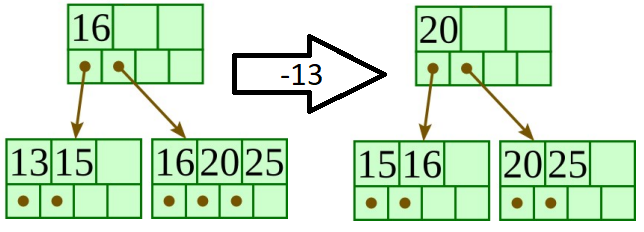
\includegraphics[width=0.5\linewidth]{b+ törlés levél}
\end{figure}

\pagebreak

\subsubsection{Belső (nem gyökér) csúcsból törlés}

\begin{outline}
	\1 Töröljük a egyesített csúcsok közötti hasító kulcsot és az egyesítés során törölt csúcsra a mutatót
	\1 Ha a csúcs tartalmaz még elég mutatót ($\lfloor d/2 \rfloor$): kész vagyunk
	\1 Ha a csúcs már túl kevés mutatót tartalmaz:
		\2 De van bal/jobb testvére, aki tud adni:
			\3 Osszuk a két testvér kulcsait és a szülőben az őket elválasztó kulcsot egyenlően
			\3 A középső kulcs a szülőben lévőt cserélje ki
			\3 A maradék menjen a két testvérbe (az kapjon többet, akinél eddig is több volt)
		\2 És nincs bal/jobb testvére, aki tudna adni:
			\3 Egyesítsük egy testvérével: először a bal oldali kulcsok, utána a két testvér szülőjében lévő elválasztó kulcs, végül a jobb oldali csúcs kulcsai jönnek
			és a jobb oldali csúcsot töröljük
			\3 Meghívunk egy törlő eljárást a szülőre: a két testvért eddig elválasztó kulcsot kell törölni (és a törölt csúcsra a mutatót)
\end{outline}

\subsubsection{Gyökérből (ami nem levél) törlés}

\begin{outline}
	\1 Töröljük a egyesített csúcsok közötti hasító kulcsot és az egyesítés során törölt csúcsra a mutatót
	\1 Ha a gyökérnek van még min 2 gyereke: kész vagyunk
	\1 Ha a gyökérnek 1 gyereke maradt: töröljük a gyökereket, a fa magassága csökken, az egyetlen gyerek lesz az új gyökér
\end{outline}

\begin{figure}[h!]
	\centering
	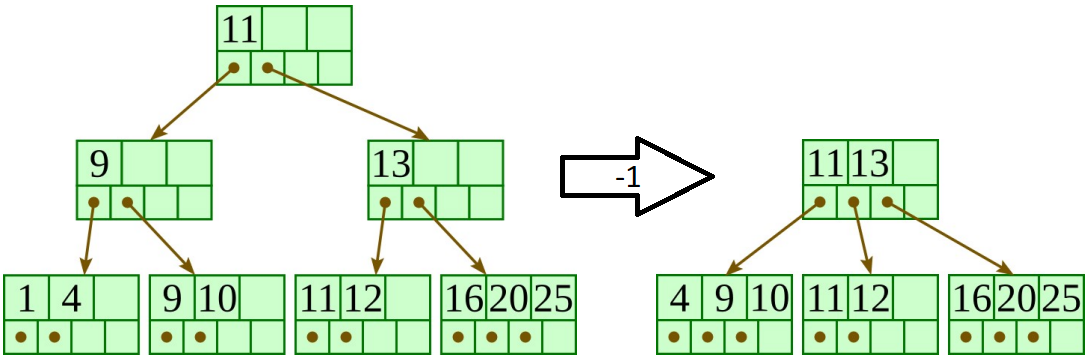
\includegraphics[width=0.8\linewidth]{b+ törlés belsőcsúcs}
\end{figure}

\end{document}
